%-----------------------------------------------------------------------------------------
\clearpage
\section{Results}
%-----------------------------------------------------------------------------------------
In the introduction I stated these aims:
\begin{itemize}
    \item To create a prototype RingTMP framework.
    \item To create a parameter server model framework.
    \item To demonstrate less communication between nodes
    \item To demonstrate that RingTMP is at least as scalable than a generic parameter
    server
    \item To demonstrate RingTMP can train neural networks to at least the same
    accuracy in at least the same amount of time as an equivalent parameter server
\end{itemize}

As can be seen in the implementation section the first two aims have been
completed. Now using experimental results it will be shown to what degree the
other aims were completed.

For experimental results we needed datasets that we could use to train the
neural networks. The first dataset chosen was the iris dataset, this is a
dataset which describes the the length and width of sepals and petals from 3
different species of flower. This dataset was chosen because of its small
feature dimension and limited examples (150), to see how well the different
network types would be effected by small feature dimension.

The second dataset used was the MNIST numbers dataset. \cite{lecun2010mnist}
This second dataset contrasts the first. Firstly this is because it has a
comparatively greater feature input of 784 (a flattened 28 by 28 image).
Secondly it a large testing and training set of 60000 training example and 10000
test examples.

Several experiments were carried out. The first experiment was training models
using the Iris dataset, this experiment was repeated 10 times for reliability
and was performed on the single node implementation of the neural network, the
parameter server implementation and the RingTMP implementation. Each
implementation used the same neural network model, consisting of 4 layers of
node numbers 4,8,8,3. The parameter server was configured with 1 server and 2
workers (3 nodes in total) and RingTMP was configured with 3 nodes 1 master 2
workers. Both these are using the same number of nodes and should represent
comparative performance. Every test session ran for at most 100 epochs, or until the
test result failed to improve for 3 epochs.

The second experiment was training models using the MNIST numbers dataset, this
experiment was repeated 5 times and was also performed on each implementation.
The neural network used in each implementation had 4 layers with a 784,50,50,10
node configuration. As before RingTMP was configured with 3 nodes as was the
parameter server. Every test session ran for at most 20 epochs, or until the
test result failed to improve for 3 epochs. But later to better compare
performance the RingTMP tests were run again with a maximum of 200 epochs.

More experiments were also performed which compared the scalability of the
parameter server with RingTMP. In these tests a 10 layer deep neural network
model was used. This has to be done as RingTMP is a model parallel framework, it
can only scale to as many layers the neural network has. Each test is repeated 5
times and changes the amount of nodes each framework uses, to see whether its
speed increases or decreases over time.

% section about training?
 

\subsection{Accuracy}

\begin{figure}[h]
    \centering
    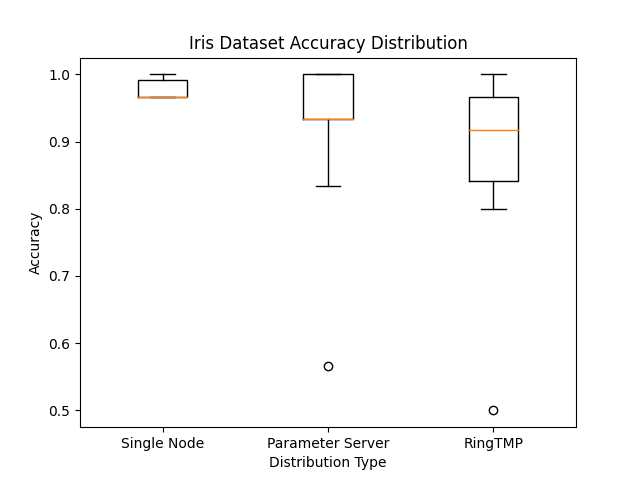
\includegraphics[width=0.45\textwidth]{iris_accuracy_boxplots}
    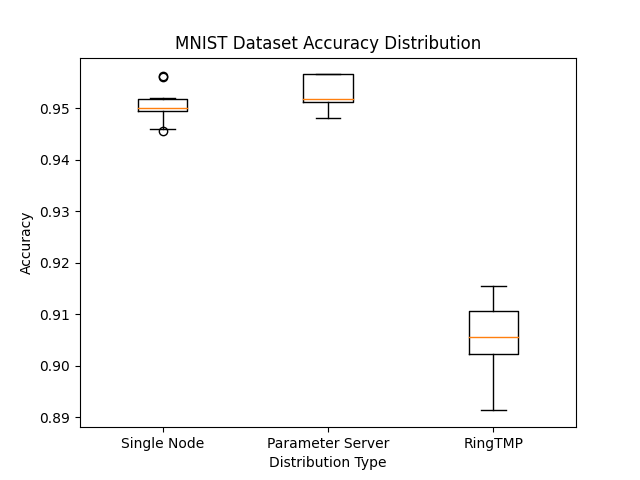
\includegraphics[width=0.45\textwidth]{mnist_accuracy_boxplots}
    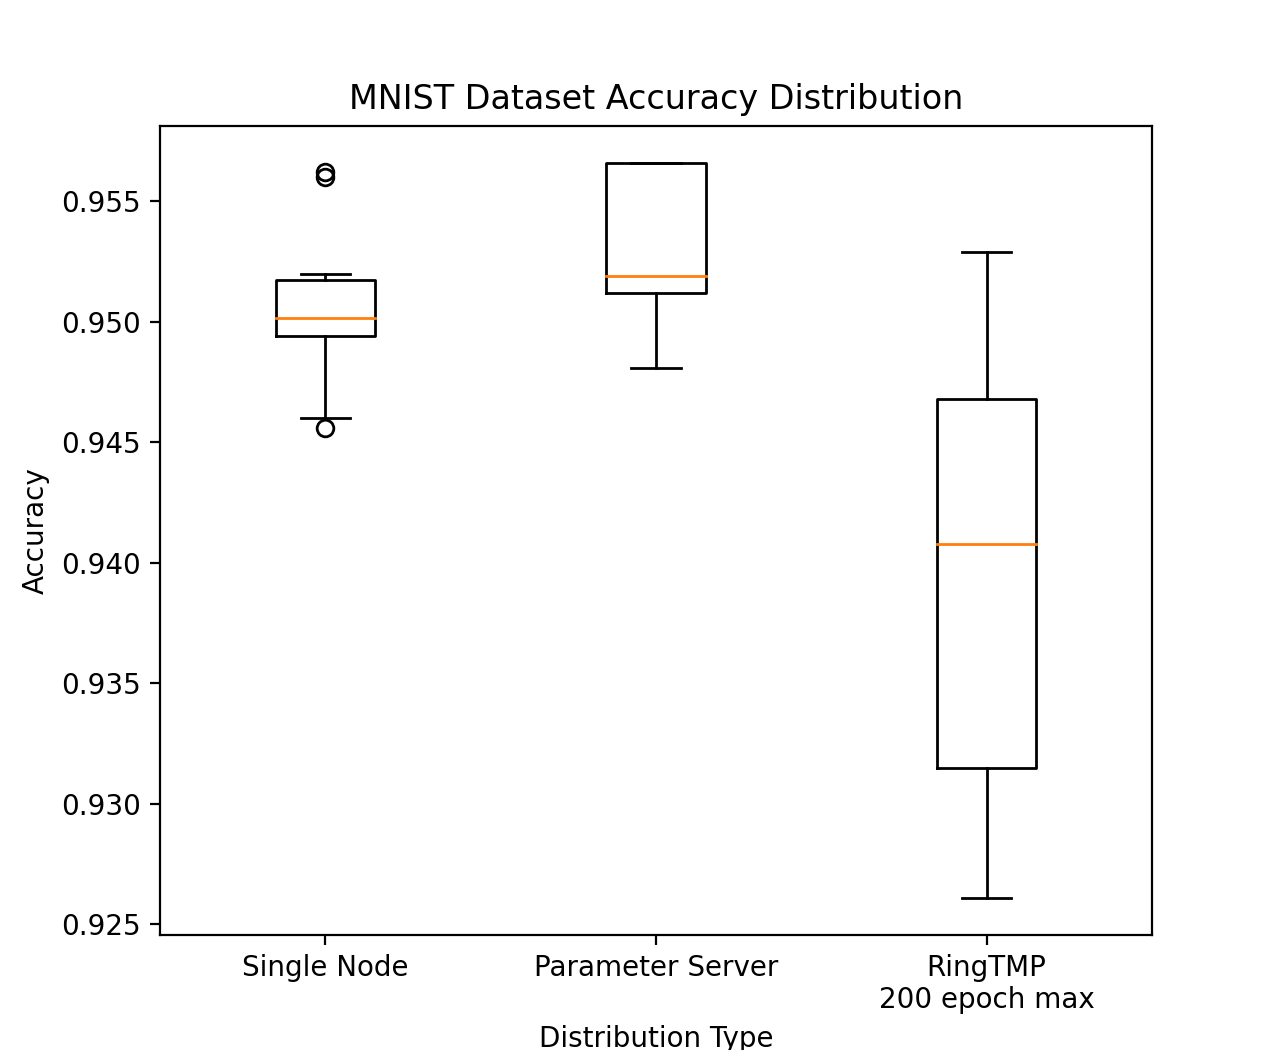
\includegraphics[width=0.45\textwidth]{mnist_accuracy_200}
\end{figure}

Here we see a box plot with the distribution of highest accuracies of each
training session for both the Iris and MNIST datasets. All distribution types
performed well on the Iris dataset each reaching a perfect score. Applying a two
tailed hypothesis Mann-Whitney U test where \(\alpha = .05\) shows that there
isn't enough statistical significant to show they are sampled from a different
population. Whereas its clear in the MNIST testing that RingTMP's accuracy was
not as high as the others. Applying the Mann-Whitney U test again shows that
Single Node and Parameter Server implementation are likely to have the same
performance distribution. RingTMP's accuracy was much lower than the other two
approaches. This was because it only took a short amount of time to complete an
epoch, but had a slower learning rate per epoch. The other two distributions
types performance often peaked before the 20th epoch as RingTMP was still
learning. To fully explore RingTMP accuracy performance, the MNIST test for
RingTMP were performed again this time with a 200 epoch limit. As you can see
from above this shows that RingTMP can achieve similar results to the single
node and parameter server implementations, albeit less frequently.

% from the same
% population, however its almost certain that RingTMP is from a different
% distribution to the first two distribution types. However the gap between the
% range is small just over 2\% difference between the two distributions. Its
% feasible that this gap could be closed with more work.

\subsection{Timings}

\begin{figure}[h]
    \centering 
    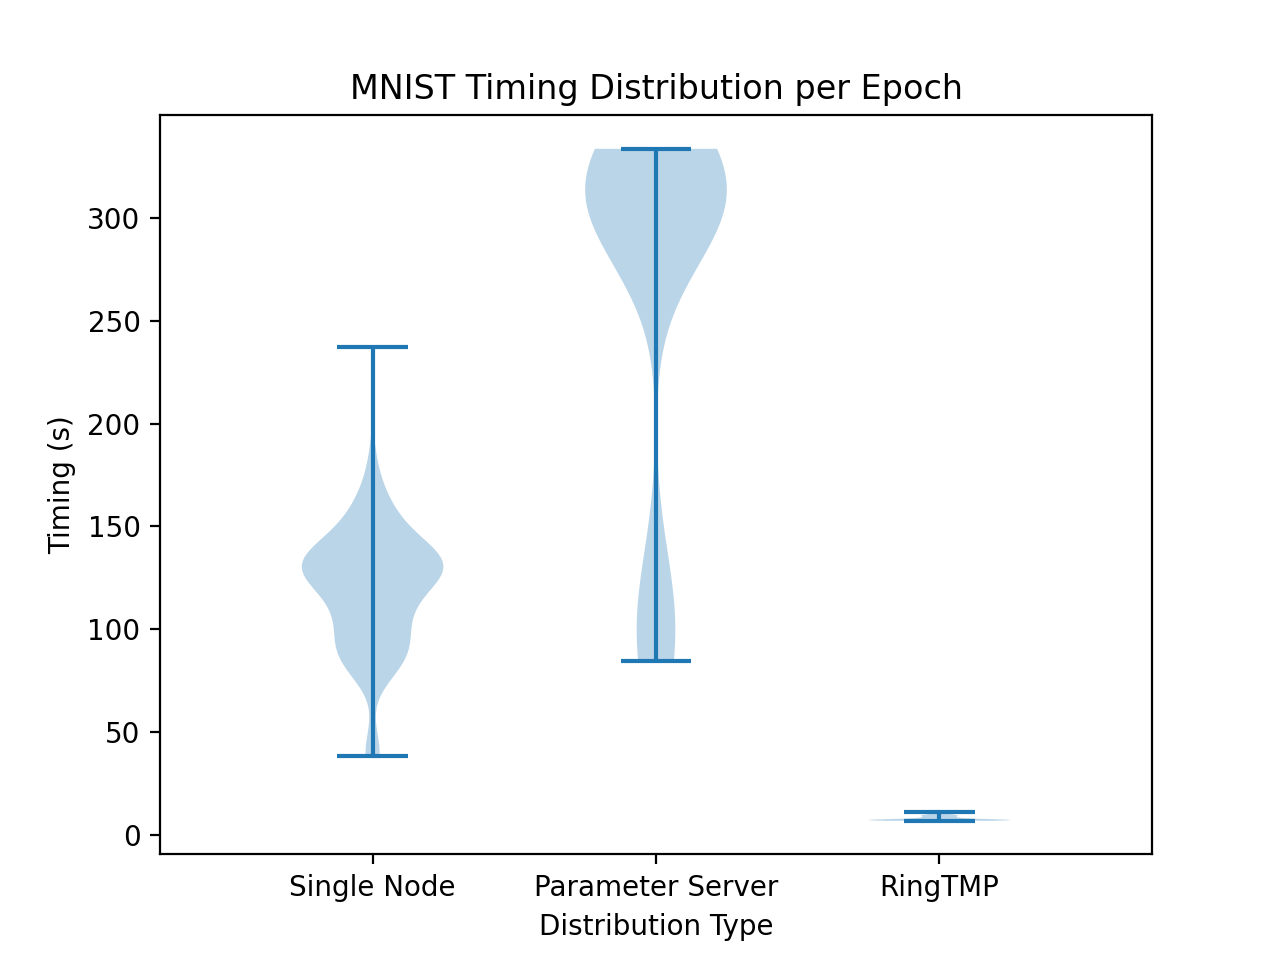
\includegraphics[width=0.49\textwidth]{mnist_timing_violinplot}
    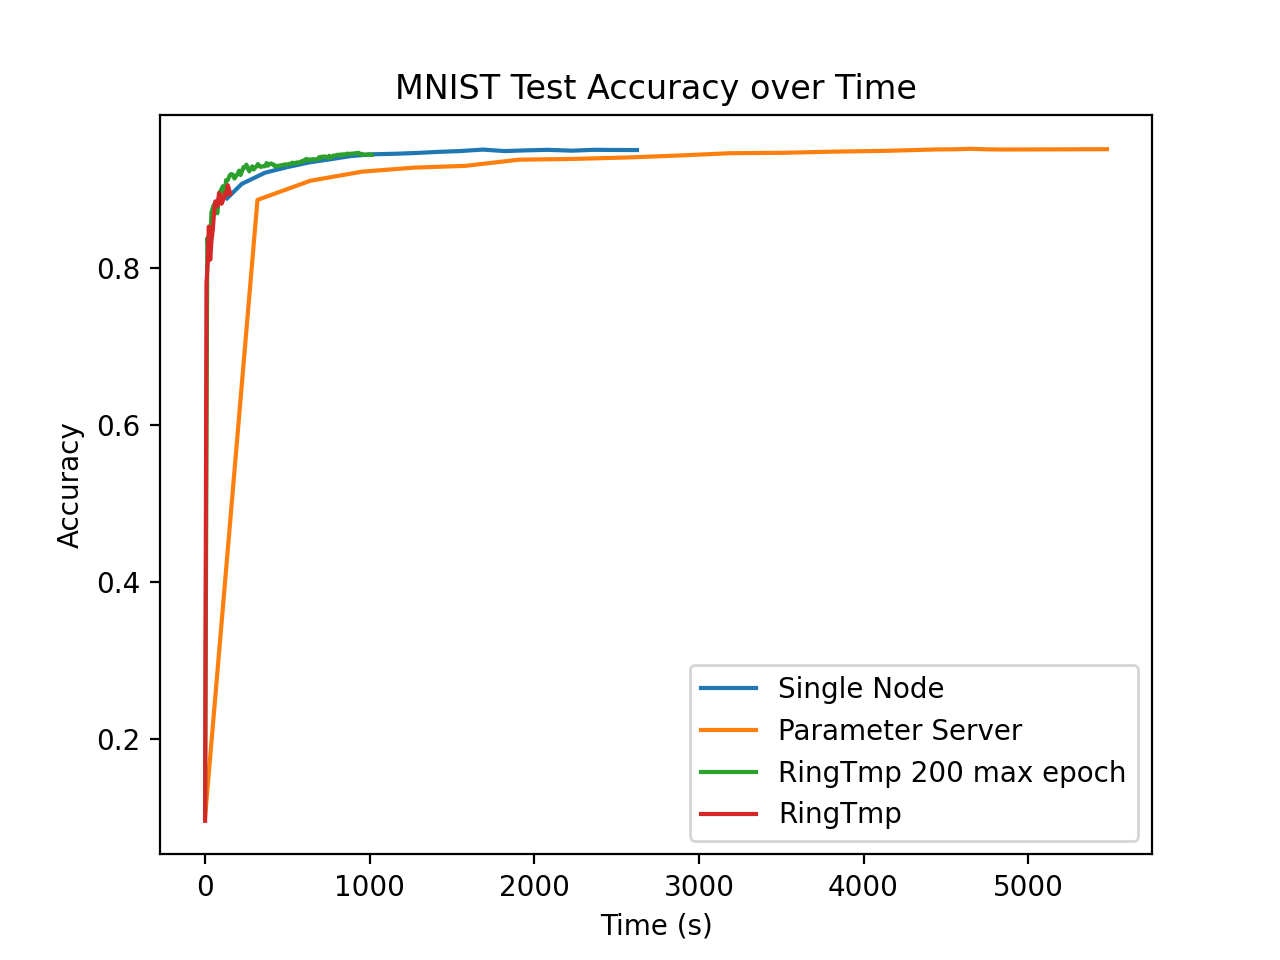
\includegraphics[width=0.49\textwidth]{mnist_accuracy_over_time}

\end{figure}

From this violin plot observe how quickly and consistently RingTMP can iterate
through each epoch (always between 7-12 seconds), this could be in part due to
the higher throughput and concurrent nature of the RingTMP network however it
must also be recognised that this may also be due to a bug. While also notice
the top heavy distribution of the parameter servers timings, more often than not
taking over 250 seconds for a single epoch, even slower than the single node
timings. Which I suspect is due to the transmission of parameters to nodes and
the time taken to aggregate parameters by the parameter server. However while
RingTMP epochs are faster, its seems to learn less from each epoch.

In the second chart of the figure we can see that RingTMP, while its learning is
a little more irratic seems to learn at the same rate as a single node, when
given a higher epoch limit. We can also see how much we were stunting RingTMP's
performance by limiting it to only 20 epochs, observe the red line being cut
short only 150 seconds into training. We can also see the parameter servers slow
rate of learning relative to the other two methods, although eventually it
achieved a higher accuracy than the other two.

\subsection{Scalability}
\begin{figure}[h]
    \centering
    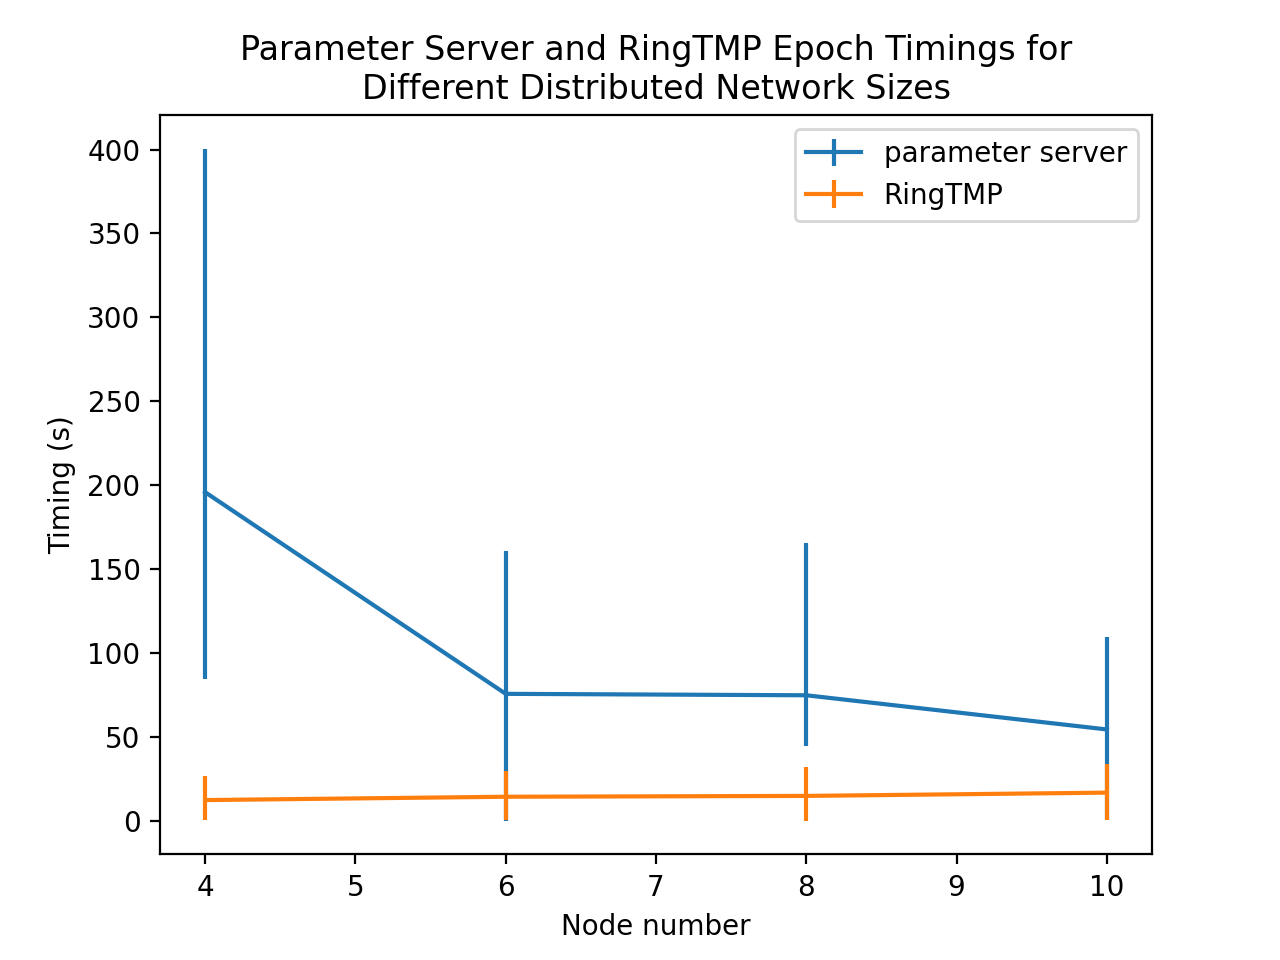
\includegraphics[width=0.6\textwidth]{scalability}
\end{figure}

To be a good distributed model, a model must be able to handle many nodes
without performance decreasing. However adding and removing nodes in each of
these models should have a different effect on the timing of epochs. We can see
that the parameter server shows a inversely proportional relationship between
the timing of an epoch and the number of nodes. However the results for the
RingTMP show a flat line. What would be expected is that the more more nodes the
model has the faster it would train, while the computation of the nodes is the
limiting factor. You could read the results of the RingTMP this way, although to
be sure you would need more evidence of the time waiting in comparison to processing.

\subsection{Communication}
\begin{figure}[h]
    \centering
    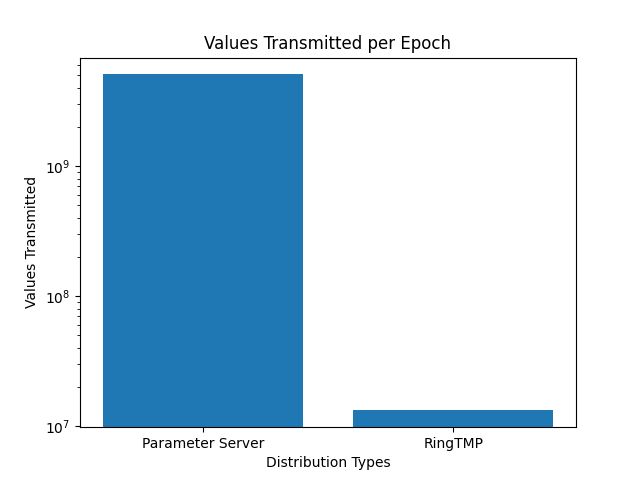
\includegraphics[width=0.49\textwidth]{comminication}
    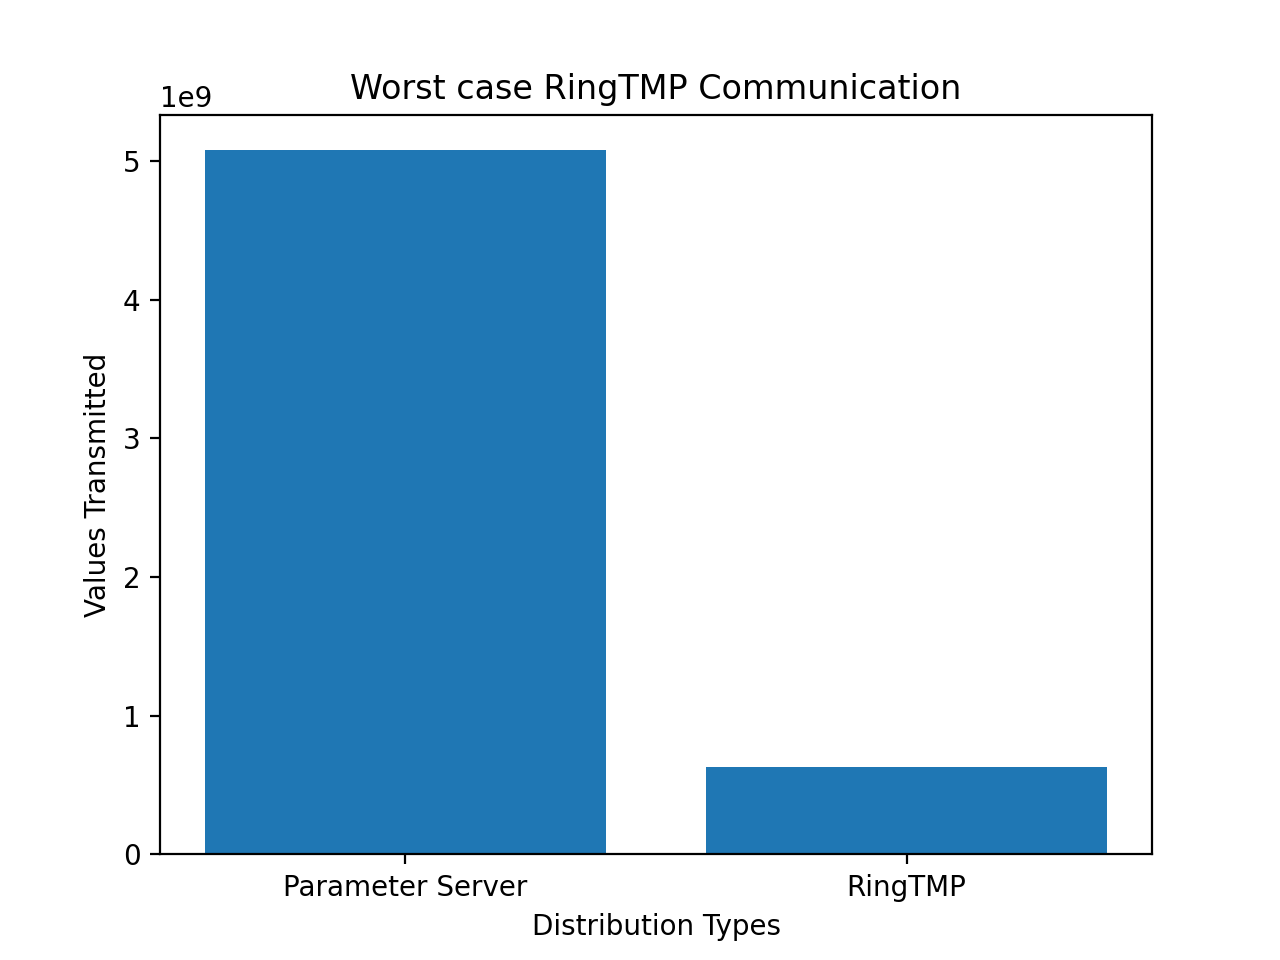
\includegraphics[width=0.49\textwidth]{worst_case_communication}

\end{figure}
On of the key goals of RingTMP was to reduce communication between nodes while
running the tests the communication of parameters and activations were being
monitored. On the right figure we can see that RingTMP has clearly achieved its
key goal of reducing communication between the nodes. Using the MNIST network of
4 layers and 784,50,50,10 node configuration it was shown that RingTMP
communicates \(1.32 \times 10^{7}\) values each epoch. However the parameter
server communicates \( 5.0772 \times 10^{9}\) each epoch, two orders of
magnitude more. However we know that RingTMP epochs are far faster than
parameter server epochs. To make a comparison about values communicated per unit
time we can take the fastest RingTMP epoch (7 seconds) and the slowest parameter
server epoch (333.5 seconds). In this case for every parameter server epoch
47.643 (3.dp) RingTMP epochs occur. Even in this most extreme situation the
RingTMP network still communicates less, as can be seen from the above figure on
the left.


\subsection{Summary}
In summary RingTMP is nearly as accurate as the Parameter Server and the Single
Node neural network. It performed similarly to the others in the Iris dataset
tests, and can achieve similar results once given the same amount of time to
train as the others. Still its clearly not as accurate as the other
implementations so this aim was not realised. However while its accuracy is not
as high as the parameter server, its rate of training, especially initially is
faster.

However there is not enough evidence to support that RingTMP is as scalable as
the parameter server, seeing as adding more nodes to RingTMP didn't produce a
reduction in time per epoch.

Most importantly its clear to see that the RingTMP framework exhibits much less
communication in comparison to a parameter server of a similar size, with the
difference being in orders of magnitude.


% In the
% parameter server we would expect the epoch time to be inversely proportional to
% the number of nodes. This is because as the nodes increase the amount of data
% given to each node decreases (e.g. 2 workers 1/2 data, 3 workers 1/3 data etc.).
% However when a node is added to RingTMP 






% In machine learning the most important metric is accuracy, more specifically the
% accuracy of correctly analysing sample it hasn't seen based on the data it
% already has. Because of this we separate our dataset into training and testing
% samples. 